\documentclass{article}

\usepackage{amsfonts}
\usepackage[utf8]{inputenc}
\usepackage[english]{babel}
\usepackage{graphicx}
\usepackage{hyperref}
\graphicspath{ {images/} }

\title{Predicting Admissions}
\author{Chinmay Sheth}
\date\today
%This information doesn't actually show up on your document unless you use the maketitle command below

\begin{document}

\maketitle

\section*{Introduction}

In this exercise, I'm analyzing a university dataset which contains information about student admissions. I am hoping to build a generalized linear model in order to reliably predict a student's admission to the university using SAS.

\section*{Dataset}

The \href{https://www.kaggle.com/mohansacharya/graduate-admissions}{dataset} that I am using was obtained from Kaggle and it contains data on university admission data. The dataset contains the following columns:

\begin{enumerate}

\item Serial No.
\item GRE Score
\item TOEFL Score
\item University Rating
\item SOP
\item LOR
\item CGPA
\item Research
\item Chance of Admit

\end{enumerate}

\section*{Data Exploration}

The dataset contains 400 entries with no data missing. The only categorical variable in the dataset is "Research" which has two values, 1 if the applicant has done research and 0 if they haven't.

\section*{Analysis}
\subsection*{Diagnostics}

Through the PROC GLM function, SAS is easily able to build a basic linear model that considers all the variables with interactions, which can be further investigated to determine to see if the linear regression assumption are met. PROC GLM is also able to differentiate between categorical and continuous variables by indicating so in the CLASS definition of the function. As such, "Research" is specified as a categorical variable in the CLASS method, and "SERIAL NO." is not included since it provides no significant meaning as they are all random.

In the diagnostic plots from Figure \ref{fig:basicmodeldiagnostics} there is a departure from the homoskedasticity assumption, that is of constant variance throughout the data, because of the decreasing variance in the data in the Residual vs Predicted Value plot and RStudent vs Predicted Value plot. There also appears to be a departure from the assumption of the expected value of the residuals to equal zero as the data in the two aforementioned plots is not centred around the horizontal zero axis. Finally, the data does not appear to be normally distributed as the Residual vs Quantile Plot shows that the points are not very closely hugging the reference line.

\subsection*{Transformations}
Using the data-driven Box-Cox technique, showed in Figure \ref{fig:boxcoxanalysis}, we can estimate the best transformation for the basic linear model which should result in diagnostic plots which have less of a departure from the linear regression assumptions. The R-Squared value has increased from 0.807246 (Figure \ref{fig:basicmodeloutput}) to 0.860190 in the transformed model, indicating that the transformed model is able to explain more variability in the predicted values than the initial model was able to. Furthermore, there appears to be a significantly less departure from the linear regression assumptions as is seen in the diagnostic plots.


\begin{figure}
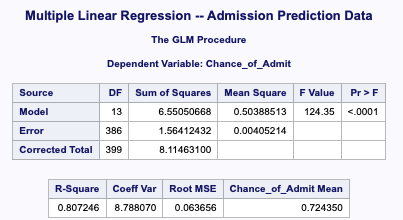
\includegraphics[scale=1]{basic_model_output.png}
\caption{Basic model output}
\label{fig:basicmodeloutput}
\end{figure}

\begin{figure}
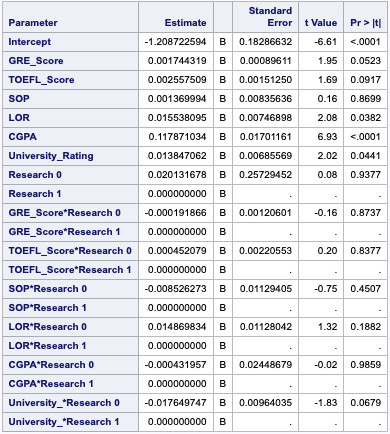
\includegraphics[scale=1]{basic_model_estimates.png}
\caption{Basic model estimates}
\label{fig:basicmodelestimate}
\end{figure}

\begin{figure}
\centering
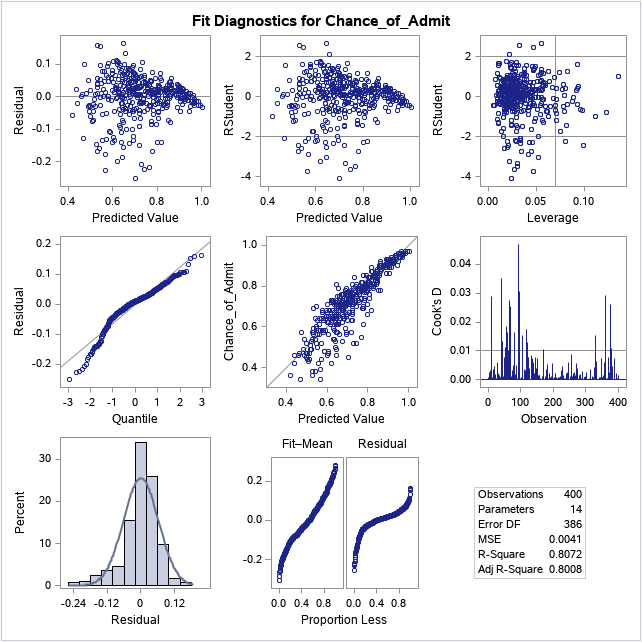
\includegraphics[scale=0.7]{basic_model_diagnostics.png}
\caption{Model Diagnostics for Basic Model with Interactions}
\label{fig:basicmodeldiagnostics}
\end{figure}

\begin{figure}
\centering
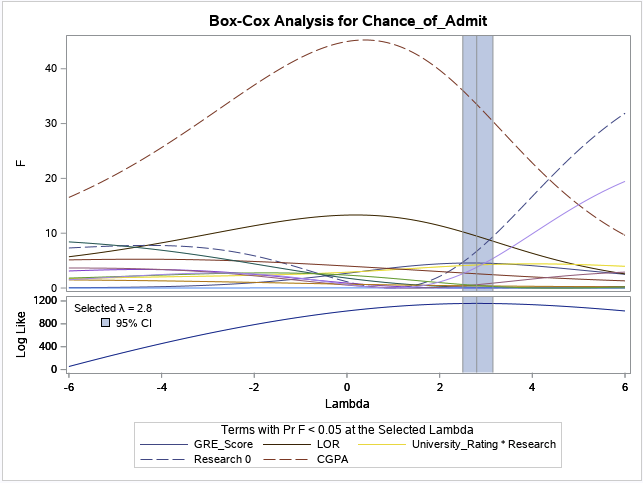
\includegraphics[scale=0.5]{box_cox_analysis.png}
\caption{Box Cox Analysis for Basic Model with Interactions}
\label{fig:boxcoxanalysis}
\end{figure}

\begin{figure}
\centering
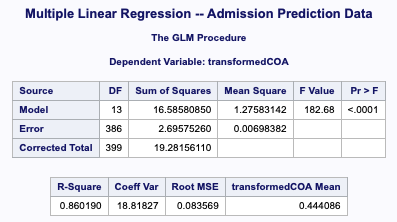
\includegraphics[scale=1]{transformed_model_output.png}
\caption{Transformed Model Output}
\label{fig:transformedmodeloutput}
\end{figure}

\begin{figure}
\centering
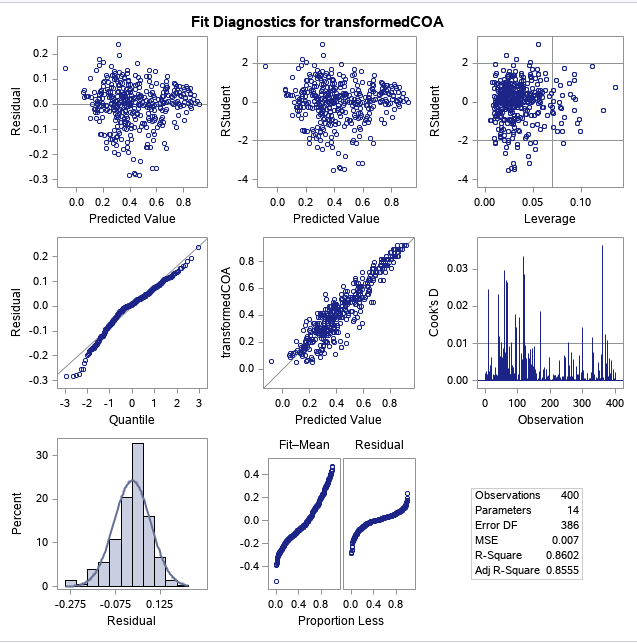
\includegraphics[scale=0.7]{transformed_model_diagnostics.png}
\caption{Transformed Model Diagnostics}
\label{fig:transformedmodeldiagnostics}
\end{figure}


\end{document}
